\chapter{Related Work}
\label{cha:sota}

%%
% \section{Top level section}

% %%%%
% \subsection{Second level section}

% %%%%%%
% \subsubsection{Third level section} 
\section{Referential Framework}
\subsection{Large Language Models}
Large Language Models (LLMs) represent a significant advancement 
in natural language processing, characterized by their ability to 
understand, generate, and interact with human language at unprecedented 
scales. Modern LLMs such as GPT-4~\cite{openai2023}, LLaMA~\cite{grattafiori2024llama3herdmodels}, 
and Claude~\cite{anthropic2023} are trained on vast corpora of text data, 
enabling them to perform a wide range of language tasks without task-specific training. 
These models have demonstrated remarkable capabilities in text generation, summarization, translation, 
and even complex reasoning tasks~\cite{brown2020}.
\subsection{Transformer Architecture}
The transformer architecture, introduced by Vaswani et al.~\cite{vaswani2023attentionneed}, forms the 
foundation of modern LLMs. Unlike recurrent neural networks, transformers process entire sequences simultaneously 
through self-attention mechanisms, allowing for more efficient training and better modeling of long-range dependencies in text. 
The architecture consists of an encoder and decoder, each composed of multi-head attention layers and feed-forward neural networks, 
enabling parallel processing and effective representation learning, as illustrated in Figure~\ref{fig:transfromer_arch}.
\begin{figure}[htbp]
    \centering
    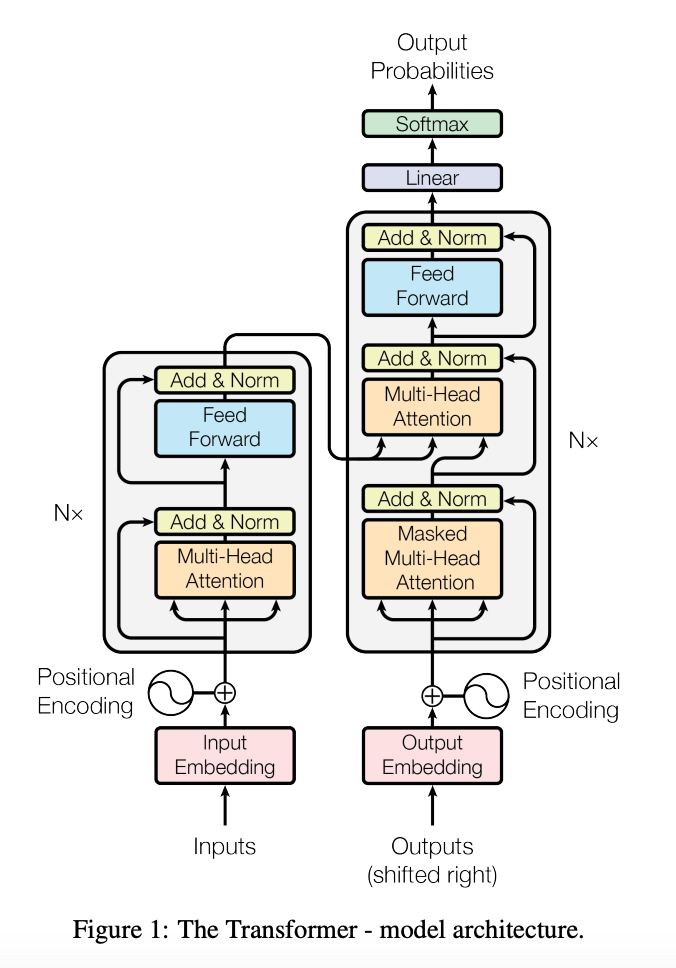
\includegraphics[width=0.7\textwidth]{figures/transformer_arch.png}
    \caption{Transformer Architecture}
    \label{fig:transfromer_arch}
\end{figure}
\subsection{Generative and Discriminative LLMs}
LLMs can be categorized as either generative or discriminative based on
their primary function. Generative LLMs, such as GPT models, focus on 
producing text by predicting the next token in a sequence given previous 
tokens. These models excel at creative writing, content generation, and
open-ended dialogue. Discriminative LLMs, in contrast, classify or 
categorize text into predefined classes or extract specific information 
from text, making them suitable for sentiment analysis, entity recognition,
and other classification tasks.
\subsection{Encoder-only, Decoder-only, and Encoder-Decoder LLMs}
The architectural design of LLMs can be categorized into three primary 
types: encoder-only, decoder-only, and encoder-decoder models.
Encoder-only models, such as BERT~\cite{devlin2019}, excel at understanding
and representing input text for classification and information extraction 
tasks. Decoder-only models, including GPT~\cite{brown2020} and 
LLaMA~\cite{grattafiori2024llama3herdmodels}, specialize in text 
generation. Encoder-decoder models, like T5~\cite{ni2021sentencet5scalablesentenceencoders} and 
BART~\cite{lewis2019bartdenoisingsequencetosequencepretraining}, combine 
both components to process input text and generate output sequences, 
making them versatile for translation, summarization, and question-answering tasks.
\subsection{Pre-training and Fine-tuning Paradigm}
Modern LLMs typically follow a two-stage development process: pre-training 
and fine-tuning. During pre-training, models learn general language 
understanding from vast unlabeled text corpora using self-supervised 
objectives such as masked language modeling or next-token prediction. 
This phase creates a foundation model with broad language capabilities. 
Fine-tuning then adapts these pre-trained models to specific downstream 
tasks using smaller, task-specific datasets. This paradigm allows for 
transfer learning, where knowledge gained from pre-training can be 
leveraged for various applications with minimal task-specific 
data~\cite{howard2018}.
\subsection{Supervised Fine-Tuning (SFT) and Reinforcement Learning from Human Feedback (RLHF)}
Supervised Fine-Tuning (SFT) involves training pre-trained models on 
labeled datasets for specific tasks. This approach uses traditional 
supervised learning methods where the model learns from input-output pairs. 
Reinforcement Learning from Human Feedback (RLHF), introduced by Christiano 
et al.\cite{christiano2017} and popularized by InstructGPT\cite{ouyang2022}, 
extends beyond SFT by incorporating human preferences into the training 
process. RLHF typically involves training a reward model based on human 
comparisons of model outputs, then using reinforcement learning to optimize 
the model's behavior according to this reward function. This approach has 
proven effective in aligning LLMs with human values and preferences, 
reducing harmful outputs, and improving helpfulness.
\subsection{Efficient Fine-tuning with LoRA and QLoRA}
As LLMs grow in size, full fine-tuning becomes computationally prohibitive. 
Low-Rank Adaptation (LoRA), introduced by Hu et al.\cite{hu2021}, offers 
an efficient alternative by freezing the pre-trained model weights and 
injecting trainable low-rank decomposition matrices into each layer of 
the transformer architecture. This approach significantly reduces the 
number of trainable parameters while maintaining performance. Quantized 
Low-Rank Adaptation (QLoRA), developed by Dettmers et al.\cite{dettmers2023}, 
further improves efficiency by combining LoRA with model quantization techniques, 
enabling fine-tuning of models with billions of parameters on consumer-grade 
hardware without sacrificing performance.
\subsection{Retrieval Augmented Generation - RAG}
Retrieval Augmented Generation (RAG), proposed by Lewis et 
al.\cite{lewis2020retrieval}, combines information retrieval with text 
generation to enhance the factuality and reliability of LLM outputs. 
RAG systems first retrieve relevant documents from an external knowledge 
base using the input query, then condition the language model's generation 
on both the input query and the retrieved documents. This approach allows 
LLMs to access information beyond their training data, reducing 
hallucinations and enabling them to cite sources explicitly. 
RAG has proven particularly valuable in knowledge-intensive domains 
such as legal analysis, where accurate reference to authoritative 
sources is essential.
\subsection{Hypothetical Document Embeddings - HyDE}
Hypothetical Document Embeddings (HyDE), introduced by Gao et al.\cite{gao2022}, 
addresses the challenge of retrieval in dense vector spaces when queries 
differ substantially from relevant documents. HyDE uses an LLM to generate a 
hypothetical document that might answer the query, then uses this document's embedding rather 
than the query's embedding for retrieval. This approach bridges the semantic gap between queries 
and documents, improving retrieval performance especially for complex or hypothetical queries. In legal 
applications, HyDE can help identify relevant precedents or regulations that may not share obvious lexical 
similarities with a user's query\cite{gao2022}.
\subsection{Prompt Engineering}
Prompt engineering encompasses techniques for formulating inputs to LLMs to 
elicit desired outputs. Effective prompts can significantly enhance model 
performance without changing model parameters. Key techniques include few-shot 
learning, where examples are provided within the prompt; chain-of-thought prompting, 
which encourages step-by-step reasoning; and system prompts that define the model's role 
and constraints. In legal applications, prompt engineering can guide models to adhere 
to specific frameworks, consider relevant factors, and produce outputs aligned with 
legal standards and practices.
\subsection{Agentic Frameworks for LLMs}
Agentic frameworks extend LLMs beyond passive response generation to enable goal-directed, 
multi-step reasoning and action. These frameworks typically involve decomposing complex 
tasks into subtasks, planning execution sequences, and monitoring progress toward goals. 
Approaches like ReAct integrate reasoning and action, while frameworks such
as AutoGPT and LangChain provide structures for autonomous task completion. 
In legal contexts, agentic frameworks can orchestrate the process of case analysis, 
from information gathering to strategy formulation and explanation.
\subsection{Evaluation Metrics for LLMs}
Evaluating LLM performance requires multiple complementary metrics. General metrics 
include perplexity, which measures how well a model predicts a sample, 
and BLEU score for comparing generated text to reference texts. 
BERTScore~\cite{zhang2020bertscoreevaluatingtextgeneration}, which uses contextual 
embeddings to measure semantic similarity between generations and references, 
offers a more nuanced evaluation of text quality. For legal applications, 
domain-specific metrics might include assessments of legal accuracy, 
procedural correctness, and citation validity. Human evaluation remains crucial, 
particularly for assessing qualities like helpfulness, clarity, and appropriateness 
of legal guidance \cite{guha2023legalbench, li2024experimentinglegalaisolutions}. 
Multi-dimensional evaluation frameworks that combine automated metrics, expert assessment, 
and layperson comprehension tests offer the most comprehensive approach to assessing legal AI systems, 
especially those intended to bridge the gap between legal professionals and the general public \cite{guo2023evaluating}. 
This holistic approach helps ensure that legal AI systems not only generate accurate and relevant 
information but also communicate it effectively to users with varying levels of legal expertise.
\subsection{Hallucinations and Bias}
LLMs are prone to hallucinations—generating content that is factually incorrect 
or unfounded—and may perpetuate or amplify biases present in their training data. 
Hallucinations pose particular challenges in legal contexts, where accuracy is 
paramount. Techniques to mitigate hallucinations include retrieval augmentation, 
which grounds generations in external knowledge sources, and uncertainty 
quantification, which helps identify when a model might be generating unreliable 
content. Addressing bias requires careful dataset curation, targeted fine-tuning, 
and ongoing monitoring of model outputs. In legal applications, these considerations 
are critical for ensuring that AI-generated guidance does not propagate systemic 
inequities or provide misleading information.

\section{State of the Art}
In Table \ref{tab:taxonomy}, an easy-to-read taxonomy of the State of the art can be found.

\subsection{Datasets}
Many of the datasets regarding legal text are limited to the English and
Chinese speaking world. This limitation extends to other jurisdictions as well, 
creating challenges for developing legal AI systems in countries like Colombia 
where access to structured legal datasets is either restricted or non-existent.
Several relevant datasets exist in the legal domain, although most focus on 
English-language jurisdictions. CaseHOLD \cite{zheng2021does} provides over 
53,000 multiple-choice questions about legal holdings, but exclusively 
covers US courts. Similarly, LegalBench \cite{guha2023legalbench} offers 
162 legal reasoning tasks across six reasoning types, yet remains primarily 
focused on common law jurisdictions. For question-answering specifically, 
AsyLex \cite{tay2023asylex} contains refugee law documents with entity 
annotations and case outcomes, while MAUD \cite{wang2023maud} focuses 
on merger agreements with expert annotations.
A notable limitation of existing datasets is their focus on professional 
legal language rather than addressing the gap between legal terminology and 
layperson understanding. While datasets contain valuable legal information, 
they don't specifically bridge legal and everyday language. The Plain English 
Summarization of Contracts \cite{manor2019plain} attempts to address this disparity 
but remains limited in scope and doesn't extend to question-answering systems for 
non-experts. LegalDiscourse \cite{spangher-etal-2024-legaldiscourse} examines when 
laws apply and who they affect but still operates within the legal language domain 
rather than translating legal concepts for laypeople.
In the retrieval domain, CLERC \cite{hou2024clercdatasetlegalcase} serves as a 
backbone for legal case retrieval and retrieval-augmented analysis generation, 
addressing the need to locate and cite relevant precedents. For multilingual 
applications, EUR-Lex-Sum \cite{aumiller-etal-2022-eur} provides legal act 
summarization across 24 European languages, though it does not address the 
Spanish-language context of Colombia.
The lack of Spanish-language legal datasets, particularly for Colombian law, 
creates a significant research gap. Existing work such as the Unfair Clause 
Detection corpus \cite{Galassi2024} demonstrates cross-lingual approaches 
for legal NLP, but does not address the specific legal structures and language 
patterns in Colombian law. The Open Australian Legal Corpus \cite{butler-2025-open-australian-legal-corpus} 
shows how comprehensive jurisdiction-specific datasets can be constructed for 
legal AI development, providing a potential template for our approach.
The creation of a specialized Colombian legal dataset is therefore necessary 
to address the specific linguistic features, legal structures, and reasoning 
patterns unique to this jurisdiction. Such a dataset would enable the development 
of legal AI systems that can effectively navigate Colombian law, making legal 
information more accessible to non-expert users in this context. Most critically, 
this dataset must bridge the gap between formal legal language and layperson 
understanding, an aspect largely overlooked in existing resources.

\subsection{Transformer-Based Models and Deep Learning}
While transformer architectures form the foundation of modern legal AI systems, 
recent research has predominantly focused on applying existing architectures rather 
than developing legal-specific modifications. Despite the remarkable performance of 
foundation models in general language tasks, architectural innovations tailored for 
legal domains remain scarce. This trend persists even as Large Language Models (LLMs) 
demonstrate significant potential for legal document processing, advice generation, and 
decision support systems.
Current implementations face persistent challenges that underscore the need for 
domain-specific adaptations. As Dahan et al.~\cite{dahan2023lawyers} emphasize, 
LLMs frequently struggle with legal precision - particularly regarding hallucination 
risks and verifiable sourcing of legal provisions. These limitations persist even as models 
grow in general capability, suggesting that architectural modifications may be necessary 
for mission-critical legal applications.
One notable exception demonstrating the value of legal-optimized architectures is the
NOMOS model by Pennisi et al.~\cite{pennisi-etal-2023-nomos}. This approach combines 
Positional Embeddings with Temporal Convolutional Networks (TCNs) to specifically address 
statutory obligation identification - a task requiring precise extraction of time-sensitive 
legal requirements from dense texts. By architecturally prioritizing temporal relationships 
in legal language, NOMOS achieves more reliable obligation extraction than generic transformers, 
suggesting pathways for future legal-specific modifications.
Later sections will explore how retrieval-augmented approaches can complement LLMs as architectural 
foundations, particularly in addressing hallucination risks through verified legal corpora.

\subsection{Retrieval-Augmented Approaches}
In contrast to more complex methods like D3LM, Retrieval-Augmented Generation
(RAG) approaches offer a compelling advantage by requiring less data and
providing more straightforward processing pipelines. While D3LM utilizes
diagnostic questions and relies on Positive-Unlabeled Reinforcement Learning
(PURL) to guide legal interactions, its process is notably intricate,
involving knowledge graphs that are highly specific to particular
legal domains. This presents a limitation when the field of expertise changes,
as the knowledge graph would need to be adjusted or rebuilt for different legal
areas.
RAG, on the other hand, bypasses this complexity by focusing on retrieving
minimal, highly relevant text segments from large legal corpora, as
demonstrated by LegalBench-RAG \cite{pipitone2024legalbenchragbenchmarkretrievalaugmentedgeneration}.
By emphasizing precise retrieval and enabling LLMs to generate accurate
citations, RAG methods allow for efficient, domain-agnostic solutions that
maintain accuracy without the overhead of domain-specific modeling. Recent
research by Manathunga et al. \cite{manathunga2023retrievalaugmentedgenerationrepresentative} has
further demonstrated RAG's potential in enhancing legal text summarization by dynamically
fetching relevant documents before generating responses. Similarly,
Lee et al. \cite{ryu-etal-2023-retrieval} explored RAG's application in case
law retrieval, showing its advantages over traditional search systems.

Many of these systems leverage FAISS (Facebook AI Similarity Search), a powerful library for 
Approximate Nearest Neighbor Search (ANNS) \cite{douze2025faisslibrary}. FAISS provides a versatile 
toolbox of indexing methods that enable efficient vector similarity searches without requiring external 
dependencies. \cite{zeng2023scalableeffectivegenerativeinformation} demonstrated that vector-based search using 
FAISS substantially outperforms keyword-driven Boolean searches in the legal domain, with measurements showing a 40\% 
reduction in the retrieval of irrelevant legal material. Similarly, \cite{panchal2025lawpalretrievalaugmented} showed 
that this vector-based approach yields better precision than traditional database query methods, allowing for faster 
response times without sacrificing the quality of results.

\subsection{Specialized Legal Question-Answering Systems}
Legal chatbots, as highlighted by Chakrabortyi~\cite{chakraborty2023revolutionizing}, 
have become powerful tools in democratizing access to legal services by 
offering cost-effective, on-demand guidance. These AI-driven systems, 
including well-known platforms such as DoNotPay and LegalZoom, 
help users draft documents and resolve disputes, although they cannot 
fully replace the nuanced expertise of human lawyers.

Works like Wu et al.'s Diagnostic Legal Large Language Model 
(D3LM)~\cite{wu2024knowledgeinfusedlegalwisdomnavigating} focus on improving LLM 
interactions with non-expert users by employing lawyer-like diagnostic 
questions to better guide legal queries. This model's use of 
Positive-Unlabeled Reinforcement Learning (PURL) significantly 
enhances the user experience by generating more relevant, targeted questions, 
ensuring that pertinent legal factors are considered during interactions 
with the LLM.

Meanwhile, Jonathan Li et al. \cite{li2024experimentinglegalaisolutions} 
introduce a human-centric approach to legal question-answering systems in 
their work, which develops the LegalQA dataset. This dataset comprises real, 
expert-curated legal questions and answers spanning diverse legal areas. 
Their research emphasizes the use of structured data and retrieval-augmented 
generation to boost LLM performance, particularly in producing factually 
correct and comprehensible answers for laypeople. This framework is an 
important step towards addressing some of the gaps found in general-purpose LLMs, 
particularly by ensuring that the legal information delivered is both accurate and 
relevant to users' needs.

\subsection{Chain-of-Thought and Reasoning Approaches}
Mavi et al. \cite{mavi2023retrievalaugmentedchainofthoughtsemistructureddomains} 
explore the Retrieval-Augmented Chain-of-Thought (CoT) model, which tackles specialized 
legal tasks by efficiently retrieving context from semi-structured data. Their model 
enhances the reasoning abilities of LLMs, especially in legal question-answering 
scenarios, by incorporating important contextual information within token limitations.

While the Chain-of-Thought (CoT) approach offers valuable step-by-step reasoning that 
improves the decision-making process in complex legal tasks, it comes with its own challenges. 
CoT relies heavily on structured reasoning, which is well-suited for certain specialized legal tasks 
but can increase the complexity of model outputs. This added complexity, especially when dealing with 
semi-structured data, can sometimes hinder scalability and efficiency when compared to the more straightforward 
retrieval and generation process of RAG. Thus, while CoT has clear benefits in enhancing accuracy for complex 
legal queries, RAG's simplicity and adaptability make it particularly advantageous for real-world applications 
where legal fields and contexts are constantly shifting.

\subsection{Addressing Hallucinations and Evaluation}
One of the most prominent problems when it comes to LLMs, especially in the legal domain, 
is the presence of hallucinations. For instance, when replying to a legal question, 
the model may generate non-existent laws or contradictory recommendations. 
The criticality of factual accuracy in legal applications makes this issue particularly concerning.
In \cite{hu2025finetuninglargelanguagemodels}, the authors address this challenge by creating a 
benchmark to systematically evaluate model hallucinations, using groundtruth law sets as reference.
Various techniques have emerged to mitigate hallucinations in legal systems, including retrieval-augmented
generation that grounds responses in verified legal sources, and uncertainty quantification methods
that help identify when a model might be generating unreliable content.

Regarding evaluation methodologies for legal AI systems, the field has evolved beyond traditional metrics
to include more specialized assessment approaches. While automated metrics such as BLEU \cite{Papineni_bleu} 
and ROUGE \cite{lin-2004-rouge} have been widely used to evaluate AI-generated legal text summaries, 
these metrics primarily measure syntactic similarity rather than legal accuracy. More recent evaluation 
frameworks incorporate BERTScore \cite{zhang2020bertscoreevaluatingtextgeneration}, which uses contextual 
embeddings to better capture semantic similarity between generated and reference texts. 

Domain-specific evaluations have also emerged, including assessments of citation accuracy, 
legal reasoning correctness \cite{guha2023legalbench}, and compliance with jurisdictional requirements.
These evaluations often focus on the model's ability to apply legal principles correctly, 
understand complex legal arguments, and provide accurate references to relevant statutes and precedents.
The evaluation of legal reasoning capabilities can be broken down into six key dimensions: problem identification, 
rule recall, rule application, rule conclusion, interpretation, and rhetorical understanding. Each dimension 
requires specific assessment methodologies and carefully curated evaluation tasks that reflect real-world legal 
scenarios while maintaining objective evaluation criteria.

A comprehensive evaluation framework for legal AI systems should encompass multiple dimensions, as suggested by \cite{guo2023evaluating}. 
This includes not only the assessment of knowledge and reasoning capabilities but also considerations of ethical alignment, 
robustness, and domain-specific performance. In the legal context, this translates to evaluating the model's ability to 
maintain consistency across different legal domains, handle complex multi-step reasoning tasks, and provide reliable 
responses under various conditions. The framework should also consider the model's capacity to recognize its limitations 
and appropriately defer to human expertise when necessary.

The effectiveness of these evaluation frameworks depends heavily on the quality and diversity of the evaluation 
data. This includes a mix of real legal documents, synthetic scenarios, and carefully curated test cases that 
cover various legal domains and complexity levels. The evaluation process should also consider the model's 
ability to handle different types of legal reasoning tasks, from straightforward rule application to complex 
interpretation scenarios, while maintaining consistency across different legal contexts and jurisdictions.

\subsection{Access to Justice and Ethical Considerations}
The practical applications of legal AI chatbots have been studied extensively 
in the context of access to justice and AI ethics. Research by \cite{chakraborty2023revolutionizing} 
highlights the potential of AI-driven legal assistants in bridging the justice gap, particularly 
in countries where legal resources are not easily accessible. This is particularly relevant for 
systems like Colombia's, where legal access disparities are significant. 

The integration of AI in legal systems brings with it significant ethical challenges, particularly 
regarding algorithmic bias. As demonstrated by \cite{Min_bias}, these systems can inadvertently 
perpetuate and amplify existing inequalities, with marginalized communities often bearing the weight 
of biased outcomes. In legal contexts, this bias can manifest through skewed legal advice, 
unequal access to information, and disproportionate impacts on vulnerable populations. The 
consequences extend beyond individual cases, potentially reinforcing systemic inequalities 
within the justice system itself.

Addressing these challenges requires a multifaceted approach that goes beyond technical solutions. 
It involves careful consideration of how training data is collected and processed, ensuring 
representation across different geographical, cultural, and socioeconomic contexts. The development 
of fairness-aware algorithms and robust accountability mechanisms becomes crucial in this context. 
These systems must be designed with human rights principles at their core, prioritizing 
non-discrimination and equal access to justice.

The work of \cite{guha2023legalbench} underscores the importance of maintaining this ethical 
focus throughout the development and deployment of legal AI systems. Their research emphasizes 
the need for evaluation frameworks that consider both technical performance and social implications, 
ensuring that these systems not only provide accurate information but also maintain fairness 
and equity in their recommendations.

\subsection{Challenges and Limitations}
The development and deployment of legal AI systems face several interrelated challenges that impact their 
effectiveness across different jurisdictions. One significant issue is the multi-jurisdictional limitations, 
where existing chatbots struggle to handle legal queries that span multiple legal systems, particularly in civil 
law countries like Colombia. This is compounded by the context processing constraints, as these systems often fail to 
effectively process long-context legal arguments, necessitating memory-intensive retrieval techniques.
Moreover, there is a notable gap in geographical datasets, with a predominant focus on English and Chinese jurisdictions. 
This creates structural disadvantages for regions with limited access to structured legal datasets, such as Colombia. 
The risk of hallucinations further undermines the reliability of LLMs in legal contexts, as they can generate non-existent 
laws or contradictory advice. This is particularly concerning given the high stakes involved in legal decision-making. Additionally, 
there is a communication gap, with most solutions failing to bridge the divide between professional legal terminology and layperson 
understanding. Traditional NLP metrics, such as BLEU and ROUGE, fall short in capturing the quality and accuracy of legal advice, 
highlighting the need for more tailored evaluation methodologies.
Addressing these challenges requires a concerted effort to optimize retrieval architectures, 
develop jurisdiction-diverse legal corpora, and create evaluation frameworks that assess factual accuracy, 
jurisdictional compliance, and layperson comprehension.

\subsection{Future Directions and Conclusions}
Building on these challenges, three key priorities emerge for advancing legal AI systems:
\begin{itemize}
    \item \textbf{RAG optimization}: Streamlined retrieval architectures show particular promise for dynamic environments like Colombia, combining citation integrity with adaptability
    
    \item \textbf{Dataset development}: Critical need for jurisdiction-diverse legal corpora, particularly Spanish-language resources for Colombian law
    
    \item \textbf{Evaluation frameworks}: Requires legal-specific metrics assessing factual accuracy, jurisdictional compliance, and layperson comprehension
\end{itemize}
The literature review demonstrates that while current systems excel in narrow legal domains, their real-world utility remains constrained 
by three fundamental gaps: (1) jurisdiction-specific knowledge gaps, (2) expert-layperson communication barriers, and 
(3) inadequate evaluation methodologies. RAG approaches currently offer the most viable path forward due to their balance 
of accuracy and adaptability, particularly when combined with targeted dataset development. The creation of a specialized Colombian 
legal corpus—incorporating both professional terminology and plain-language explanations—would simultaneously address dataset scarcity 
and communication gaps while providing a testbed for improved evaluation frameworks. This positions Colombia as a strategic proving ground 
for next-generation legal AI systems that prioritize accessibility alongside technical capability.

\begin{table}[h]
    \centering
    \caption{Taxonomy of Legal AI Literature}
    \label{tab:taxonomy}
    \setlength{\tabcolsep}{4pt} % Reduce column padding
    \begin{tabular}{p{3.2cm}p{3.8cm}p{6cm}} % Adjusted column widths
    \toprule
    \textbf{Category} & \textbf{Subcategory} & \textbf{Papers} \\
    \midrule
    
    % --- Datasets Section ---
    \multirow{5}{*}{Datasets} 
    & English Legal Datasets & 
    \begin{tabular}[t]{@{}p{\linewidth}@{}}
    \cite{zheng2021does} - CaseHOLD \\
    \cite{guha2023legalbench} - LegalBench \\
    \cite{tay2023asylex} - AsyLex \\
    \cite{wang2023maud} - MAUD \\
    \cite{butler-2025-open-australian-legal-corpus} - Open Australian Legal Corpus
    \end{tabular} \\
    \cline{2-3}
    
    & Multilingual Legal Datasets & 
    \begin{tabular}[t]{@{}p{\linewidth}@{}}
    \cite{aumiller-etal-2022-eur} - EUR-Lex-Sum \\
    \cite{Galassi2024} - Unfair Clause Detection
    \end{tabular} \\
    \cline{2-3}
    
    & Legal-Layperson Bridging & 
    \begin{tabular}[t]{@{}p{\linewidth}@{}}
    \cite{manor2019plain} - Plain English Summarization \\
    \cite{spangher-etal-2024-legaldiscourse} - LegalDiscourse
    \end{tabular} \\
    \cline{2-3}
    
    & Legal Case Retrieval & 
    \cite{hou2024clercdatasetlegalcase} - CLERC \\ 
    \midrule
    
    % --- Transformer Models ---
    \multirow{2}{*}{Transformer-Based} 
    & Pre-trained Models & 
    \cite{liu2019robertarobustlyoptimizedbert} - RoBERTa \\ 
    \cline{2-3}
    
    & Domain-Specific Models & 
    \begin{tabular}[t]{@{}p{\linewidth}@{}}
    \cite{pennisi-etal-2023-nomos} - NOMOS \\
    \cite{dahan2023lawyers} - Lawyers and LLMs
    \end{tabular} \\ 
    \midrule
    
    % --- Retrieval Approaches ---
    \multirow{2}{*}{Retrieval-Augmented} 
    & RAG Systems & 
    \begin{tabular}[t]{@{}p{\linewidth}@{}}
    \cite{pipitone2024legalbenchragbenchmarkretrievalaugmentedgeneration} - LegalBench-RAG \\
    \cite{manathunga2023retrievalaugmentedgenerationrepresentative} - RAG Summarization \\
    \cite{ryu-etal-2023-retrieval} - Case Law RAG \\
    \cite{panchal2025lawpalretrievalaugmented} - LawPal
    \end{tabular} \\
    \cline{2-3}
    
    & Similarity Search & 
    \cite{zeng2023scalableeffectivegenerativeinformation} - FAISS Retrieval \\ 
    \midrule
    
    % --- QA Systems ---
    \multirow{2}{*}{Specialized Legal QA} 
    & Legal Chatbots & 
    \cite{chakraborty2023revolutionizing} - Legal Chatbots \\ 
    \cline{2-3}
    
    & Diagnostic Systems & 
    \begin{tabular}[t]{@{}p{\linewidth}@{}}
    \cite{wu2024knowledgeinfusedlegalwisdomnavigating} - D3LM \\
    \cite{li2024experimentinglegalaisolutions} - LegalQA
    \end{tabular} \\ 
    \midrule
    
    % --- COT ---
    Chain-of-Thought & RAG-CoT Integration & 
    \cite{mavi2023retrievalaugmentedchainofthoughtsemistructureddomains} - RAG-CoT \\ 
    \midrule
    
    % --- Evaluation ---
    \multirow{2}{*}{Evaluation} 
    & Metrics & 
    \begin{tabular}[t]{@{}p{\linewidth}@{}}
    \cite{Papineni_bleu} - BLEU \\
    \cite{lin-2004-rouge} - ROUGE
    \end{tabular} \\ 
    \cline{2-3}
    
    & Hallucination Detection & 
    \cite{hu2025finetuninglargelanguagemodels} - Hallucination Benchmark \\ 
    \midrule
    
    % --- Ethics ---
    AI Ethics & Bias Mitigation & 
    \cite{Min_bias} - Bias Detection \\ 
    \midrule
    
    % --- Research Tools ---
    Legal Research Tools & NLP Systems & 
    \cite{Singh_legal} - AI Legal Research \\ 
    \bottomrule
    \end{tabular}
    \end{table}



% \subsection{Domain-Specific LLMs for Legal and Regulatory Text}
% In \cite{martinez-etal-2025-scalable}, where we present a comprehensive approach to 
% developing LLMs tailored specifically for understanding regulatory texts. 
% Our methodology involves constructing a specialized corpus through 
% large-scale scraping of financial and regulatory documents across domains 
% like compliance, licensing, and financial reporting. By preprocessing this 
% data with GPT-4o-mini and further pre-training a LLaMA-3.1-8B model on the 
% curated corpus, we demonstrate improved capability in tasks such as acronym 
% expansion and regulatory question-answering. Our implementation of 
% Quantized Low-Rank Adaptation (QLoRA) addresses computational 
% efficiency concerns while maintaining model performance. 
% Although our model shows only slight improvements over baseline in some tasks, 
% particularly in named entity recognition, this approach illustrates the 
% potential of domain-specific LLMs in regulatory text interpretation and 
% establishes a foundation for specialized NLP evaluation methodologies. 
% This scalable framework offers a balanced alternative between computational 
% requirements and performance, allowing potential deployment on more accessible 
% hardware compared to larger models, making it particularly relevant for contexts 
% where computational resources may be limited, such as Colombia's legal system.
% Future developments in multilingual legal AI, enhanced retrieval mechanisms, and 
% AI-powered contract analysis will be crucial in making legal AI tools more accessible, 
% reliable, and widely applicable in legal practice, particularly in diverse jurisdictions 
% like Colombia where multiple language variations and regional legal nuances may exist.
\endinput

